\section{RECESO Architecture}
\label{sec:proposal}

The general architecture of RECESO is shown in Figure \ref{fig:arquitecture}. It is mainly composed by four modules, supported by ontologies that model the knowledge related to users' preferences, context factors, and POI:  
%In this section we describe the architecture and functioning of our proposed User-Driven and Context-aware Hybrid Recommender System. Figure \ref{fig:arquitecture} shows its components:
\begin{itemize}
    \item \textbf{Data Gathering Module}: User's preferences are received by the system, explicitly (i.e., direct interaction) or implicitly (e.g., data mining, social networks analysis, user's pictures analysis). These preferences are related to categories of POI, according to the POI ontology. 
    \item \textbf{User Interest Module}: User's preferences are propagated from higher classes to lower classes of the POI ontology.
    \item \textbf{Context Module}: The system receives information about the context of the user, explicitly or implicitly (retrieved from an API, mobile information, etc.).
    \item \textbf{Recommendation Module}: The system recommends a set of places to the user.
\end{itemize}

% Regarding the ontology  \textcolor{red}{????}
      
In the following sections, we describe in detail each module.


\begin{figure}[h]
\centering
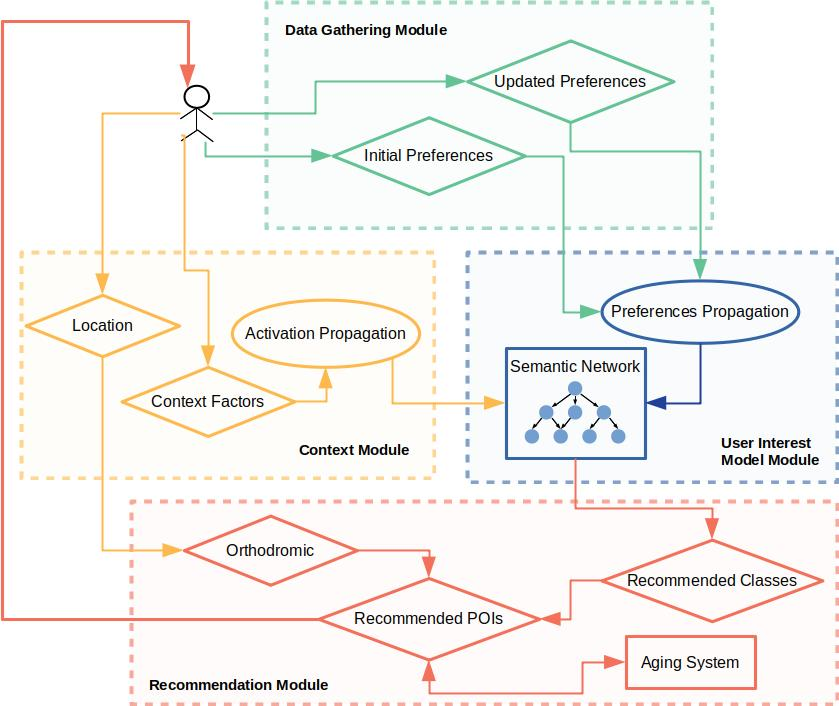
\includegraphics[scale=0.4]{draws/arquitecture.jpg}
\caption{System architecture}
\label{fig:arquitecture}
\end{figure}

\subsection{Data Gathering Module}
Initially, the system receives or calculates
%should receive 
initial \textbf{preferences}, as 
%real 
values between $0$ and $1$, for the higher classes of the POI ontology. To obtain these values, the user could explicitly set them by interacting with the system or they could be implicitly determined using data mining, social network analysis, geo-data, similar profile users, friends preferences, etc. During the lifetime of the system, users' preferences are updated, according their behaviors. 
%the user can feed new updated preferences to the system.

\subsection{User Interest Model Module}
Inspired on the work of Bahramian et al. \cite{bahramian_abbaspour_claramunt_2017}, we introduce the concept of \textbf{semantic network}: a tourism ontology extended with the user's preferences (see Figure \ref{fig:initial_pref}) and context factor links
(see Figure \ref{fig:init_act}). Just like Bahramian et al. \cite{bahramian_abbaspour_claramunt_2017}, we take advantage of the hierarchical shape of the semantic network for propagating the preference of superclasses to subclasses. Alongside preferences, each node of the semantic network has a \textbf{confidence} related to the user, a value between $0$ and $1$ that defines how sure is the system that the computed preference is the real one, i.e. a weight that is near $1$ if the computed preference is probable to be the actual user's preference, and near $0$ if it is not. When a preference is explicitly given by the user, its confidence is $1$, but when it is inferred from its ancestors or other kind of analysis, its confidence should be less than $1$. 

For each user, we compute the preference $pref_c$ and the confidence $conf_c$ of each class $c$, according to Eq. (\ref{eq:preference}) and Eq. (\ref{eq:confidence}), respectively; 
where $ancestors(c)$ is the set of ancestors of the ontology class $c$, $pref_p$ is the user's preference of the class $p$, $conf_p$ is the confidence about the user's preference for
class $p$, and $\alpha$ is the \textit{decrease rate} indicating
how much should decrease the \textit{confidence} at each level. 

\begin{equation} \label{eq:preference}
    pref_c = \frac{\displaystyle \sum_{p \in ancestors(c)}{conf_p pref_p}}
    {\displaystyle  \sum_{p \in ancestors(c)} {conf_p}}
\end{equation}
\begin{equation} \label{eq:confidence}
    conf_c = \frac{\displaystyle \sum_{p \in ancestors(c)} {conf_p}}{|ancestors(c)|} - \alpha
\end{equation}

These calculations are applied to each node traversing from the higher classes, whose preferences are obtained from the Data Gathering Module, to the \textit{sinks}, while decreasing confidence values and therefore preference values. 
This process is called \textbf{preference propagation}. 

Figure~\ref{fig:initial_pref} shows an example of initial preferences gathered with values $0.85$, $0.5$ ,and $0.7$ for the 
%initial 
ontology classes \textit{Cultural}, \textit{Store}, and \textit{Sport}, respectively. The initial confidence for each preference is $1$, since they are gathered explicitly from the user. Then, Figure~\ref{fig:pref_prop} shows the preference propagation with these values, applying Eq. (\ref{eq:preference}) and Eq. (\ref{eq:confidence}), with $\alpha = 0.1$.

\begin{figure}[h]
\centering
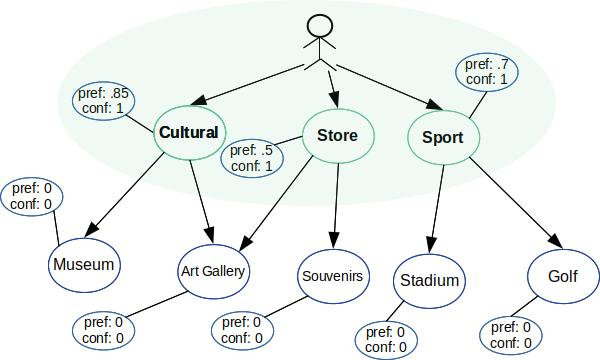
\includegraphics[scale=0.5]{draws/initial_pref.jpg}
\caption{Initial preferences for {\tt Cultural, Store}, and {\tt Sport} classes}
\label{fig:initial_pref}
\end{figure}

\begin{figure}[h]
\centering
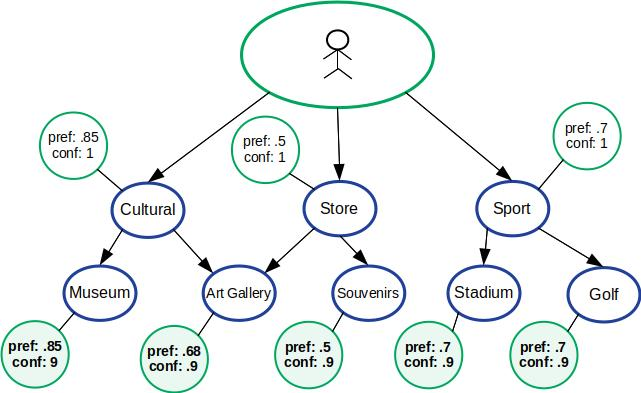
\includegraphics[scale=0.5]{draws/pref_spred.jpg}
\caption{Preference propagation for {\tt Museum, Art Gallery, Souvenirs, Stadium}, and {\tt Golf} classes, with 0.1 as decrease rate ($\alpha$=0.1)}
\label{fig:pref_prop}
\end{figure}

\subsection{Context Module}
We define the \textbf{activation} of a node of the semantic network (a POI) as the value that determines how feasible 
is the user to visit a place that belongs to the category of  node's ontology class, according to the current user's context.
The user's context is determined by the \textbf{context factors}, which are entities that describe the characteristics of the user’s context that could affect their decision to go to a specific place. The context factors could be time, day, weather, transportation, mood, etc. To make a recommendation, the system has the
values for each context factor per user ($contextFactors$ set), obtained either explicit (provided by users) or implicit (deduced by historical behaviors, data mining, etc.).  For example, in Figure \ref{fig:init_act} the context values obtained are \textit{cloudless, night} and \textit{weekend}.

Let's define $f_x$ the \textit{fulfillment} of a context factor value $x$, where $f_x = 1$ if $x$ fulfills or $f_x = 0$ otherwise. Let's also define $r_{c,x}$ as the \textit{relevance} of $x$ for the node $c$, which is a value in $[0, 2]$ that specifies how much the context factor value can affect the user's decision to go to a POI in $c$'s ontology class; a value of $1$ means indifference; a value near $2$ means the fulfillment increases the wish to go to the POI; a value near $0$ means the fulfillment decreases the wish to go the POI. Hence, we define $act_c$ as the activation for a node $c$ which is directly linked to the user's context factors values ($contextFactors$), as shown in Eq. (\ref{eq:high_activation}), and the activation for internal nodes is defined in Eq. (\ref{eq:activation}), calculated using the higher classes.


\begin{equation} \label{eq:high_activation}
    act_c = \sum_{x \in contextFactors} r_{c,x} f_x
\end{equation}

%and the activation for the internal nodes is defined as follows:

\begin{equation} \label{eq:activation}
    act_c = \frac{\displaystyle \sum_{c' \in ancestors(c)} act_{c'}}{|ancestors(c)|}
\end{equation}.

%These formulas are used for an \textbf{Activation propagation} from the higher classes. 
Figures \ref{fig:init_act}, \ref{fig:high_act} and \ref{fig:spread_act} show an example, where:

\begin{itemize}
    \item $r_{Cultural, cloudless} = 1$
    \item $r_{Cultural, night} = 0.5$
    \item $r_{Cultural, weekend} = 1.8$
    \item $r_{Store, cloudless} = 1.5$
    \item $r_{Store, night} = 1.3$
    \item $r_{Store, weekend} = 1$
    \item $r_{Sport, cloudless} = 2$
    \item $r_{Sport, night} = 0.2$
    \item $r_{Sport, weekend} = 1.5$
    \item $f_{cloudless} = f_{night} = f_{weekend} = 1$
    \item $f_x = 0$, $x \notin \{cloudless, night, weekend\}$
\end{itemize}

First, the system receives the context of the user, which in this example is a {\it cloudless night on the weekend} (Figure \ref{fig:init_act}). Then, using Eq. (\ref{eq:high_activation}), the activation values for \textit{Cultural}, \textit{Store}, and \textit{Sport} are computed (Figure \ref{fig:high_act}). Finally, using Eq. (\ref{eq:activation}), the activation values for \textit{Museum}, \textit{ArtGallery}, \textit{Souvenirs}, \textit{Stadium}, and \textit{Golf} are computed (Figure \ref{fig:spread_act}).

\begin{figure}[h]
\centering
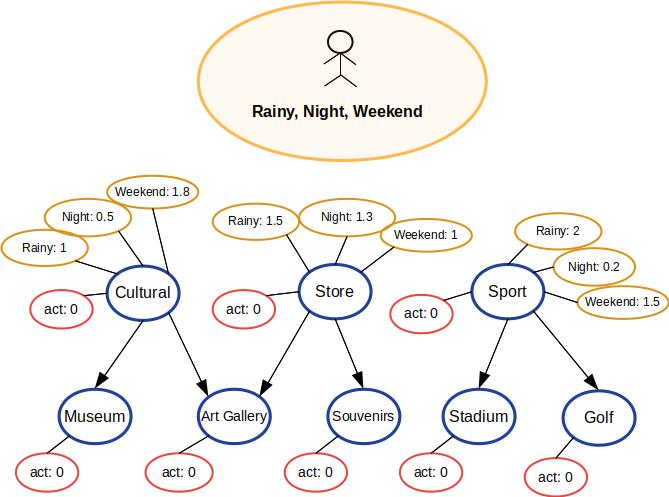
\includegraphics[scale=0.45]{draws/initial_act.jpg}
\caption{System receives {\tt sunny, night, weekend} as user context}
\label{fig:init_act}
\end{figure}


\begin{figure}[h]
\centering
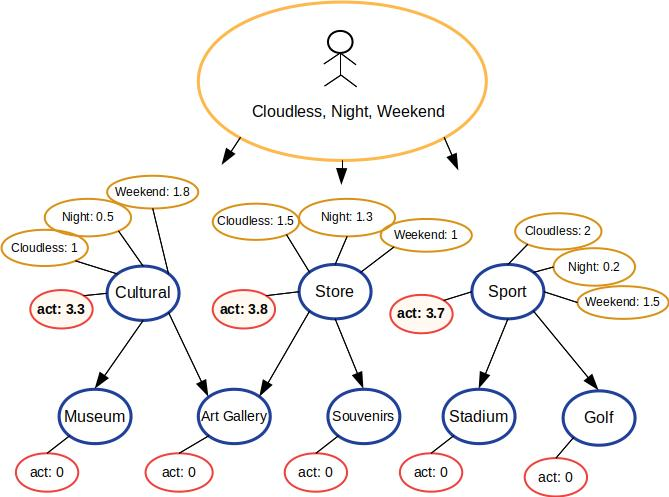
\includegraphics[scale=0.45]{draws/high_act.jpg}
\caption{Compute activation for {\tt Cultural, Store}, and {\tt Sport} classes}
\label{fig:high_act}
\end{figure}

\begin{figure}[h]
\centering
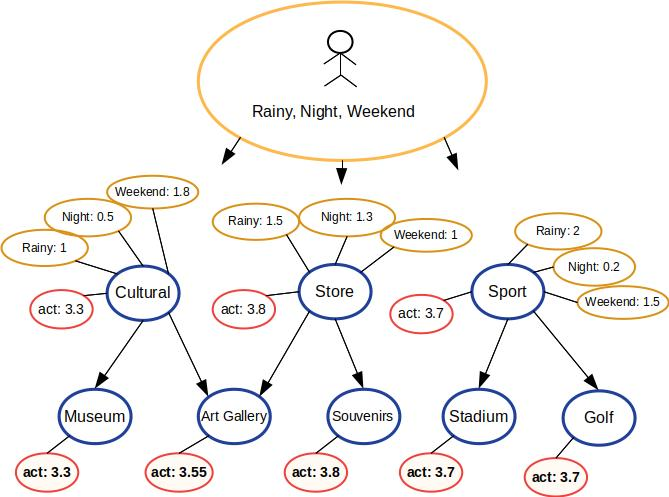
\includegraphics[scale=0.45]{draws/spread_act.jpg}
\caption{Spread activation to {\tt Museum, Art Gallery, Souvenirs, Stadium}, and {\tt Golf} classes}
\label{fig:spread_act}
\end{figure}

Furthermore, this module receives the user's \textbf{location}, which will be used for querying near POI.

\subsection{Recommendation Module}

%We will first give two necessary definitions to compute the final score of an item and then we give the formula.

Besides user's preferences related to POI and context factors, the system bases the recommendations on  an {\it aging-like} algorithm,  to ensure serendipity, on the distance of the POI to the user's location and its transportation medium, and on calculated scores of POI. In the following, we explain these three functionalities.

\subsubsection{\bf Aging System}

Let's define $\eta_p$ as the POI $p$'s aging, initialized as $\eta_p = 1$. Let's define $H$ as the \textit{aging rate}. Each time a POI $p$ is recommended to the user, $\eta_p$ decreases by $H$. When $\eta_p < 0.1$, $\eta_p$ is reset to $1$. 

\subsubsection{\bf Great-Circle distance}
Since the euclidean distance between two points on Earth would cross through the surface, we should use a more convenient measurement of distance: the \textit{great-circle distance} or \textit{orthodromic distance}. It is the shortest distance, along the surface of a sphere, between two points on the surface of the sphere. It is measured with circles on the sphere whose centers coincide with the center of the sphere. Those circles are called \textit{great-circles}. If we assume Earth is a perfect sphere and hence use Great-Circle distance, we get distances with errors no more than $0.5\%$, according to \cite{1997admiralty}. 

The distance between two points $i$ and $j$ on a sphere of radius $r$ is computed as shown in Eq. (\ref{eq:gc-dist}).
%with the following formula:
\begin{equation} \label{eq:gc-dist}
    \begin{split}
        \scriptstyle{dist_{i,j} \ = \ r \cdot arccos (} & \scriptstyle{cos(lat_i) \cdot cos(lat_j) \cdot cos(lon_i - lon_j)} \\
                                        & \scriptstyle{+ \ sin(lat_i) \cdot sin(lat_j) )}
    \end{split}
\end{equation}

\subsubsection{\bf Score} \label{section:score}
The system calculates the \textit{score} of each instance $p$ of a class $c$ in  the ontology, in terms of user's preferences (Eq. (\ref{eq:preference})), activation level (Eq. (\ref{eq:high_activation}) or Eq. (\ref{eq:activation})), the aging value ($\eta_p$), and the great-circle distance. Eq. (\ref{eq:score}) shows how the \textit{score} is calculated; where $w_i$ are configuration parameters of the system that represent the weigh of each term ($\sum w_i =1$), $pref_c$ is the user's preference on the class $c$, $act_c$ is the activation level of class $c$, $\eta_p$ is the aging factor, $dist_{u,p}$ is the great-circle distance between user's location and POI $p$, and $maxdist$ is the maximum great-circle distance that a $p$ should be from user $u$  (this distance depends on the user transportation that can be detected  from the user's smartphone sensors, for example).

%Let each $k_i$ be a parameter to the system \textcolor{red}{Cuales parametros?}, $dist_{u,p}$ be the great-circle distance between user $u$ and POI $p$, and $c$ be the node whose class is the one to which $p$ belongs to. We define the \textit{score} of $p$ as a function that receives the maximum great-circle distance that a $p$ should be from $u$ as follows \textcolor{red}{Como podemos agregar aqui que esa max distancia dependerá del medio de transporte del usuerio?}:

\begin{equation} \label{eq:score}
    \begin{split}
        %score_p(maxdist) = 
score_p =   \ &w_1 \cdot pref_c + w_2 \cdot act_c \\
                                        &+ w_3 \cdot \eta_p - w_4 \cdot \frac{dist_{u,p}}{maxdist}
    \end{split}
\end{equation}

The system uses this score for returning the list of "top places", whose length could be configured.

\subsection{User interface (Client)}
This system could be interacted with mobile apps, web apps, or any other suitable \textit{front-end}, which should be in charge of supporting PULL (user explicitly asks for a recommendation) or PUSH (\textit{front-end} gathers information to send to the system, which then returns the recommendation) paradigms.



